\section{How it works}
This section describes how self-propelled instrumentation works from user's
perspective. Each subsection is a major step in the workflow.

\subsection{Building Agent}
Users build their own {\em Agent} shared library using self-propelled
instrumentation's API.
\begin{enumerate}
\item Coding. Users need to write two pieces of code: 1) payload function; 2)
  configuration code that registers payload function and does some customization
  and configuration. The configuration code must be executed right away when the
  {\em Agent} shared library is loaded into the application process, so the
  configuration code should be in the init function of the {\em Agent} shared
  library, i.e., the function with gcc directive
  \_\_attribute\_\_((constructor)).
\item Building. Users build the code into an {\em Agent} shared library linking
  with {\em libagent.so} provided by the self-propelled instrumentation
  infrastructure.
\end{enumerate}

\subsection{Injection}
Users run {\em Injector} in command line. They specify in command line arguments
the path of an {\em Agent} shared library and the application process to inject
to.

One trick to check whether the {\em Agent} shared library is injected
successfully is to look at memory maps file of the application process, i.e.,
/proc/PID/maps.

\subsection{Initialization} %changed configuration to initialisation as

The initialisation code is executed right away when {\em Agent} shared library
is loaded into the application process.
It tells self-propelled instrumentation what are payload functions provided by
users, how would initial instrumentation be done, whether or not to enable
inter-process instrumentation propagation etc.

\subsection{Initial Instrumentation}
Once the configuration code in the {\em Agent shared library} finishes execution
inside the application process, the initial instrumentation would be performed
right away, e.g., instrumenting all function calls inside the {\em main}
function.

\subsection{Instrumentation Propagation}
When one of the initial instrumentation gets executed, then instrumentation
propagates itself either within the process by following control flow, or across
process boundaries by following communication flow.

\subsubsection{Intra-process propagation}
\begin{figure}[ht]
  \centering
  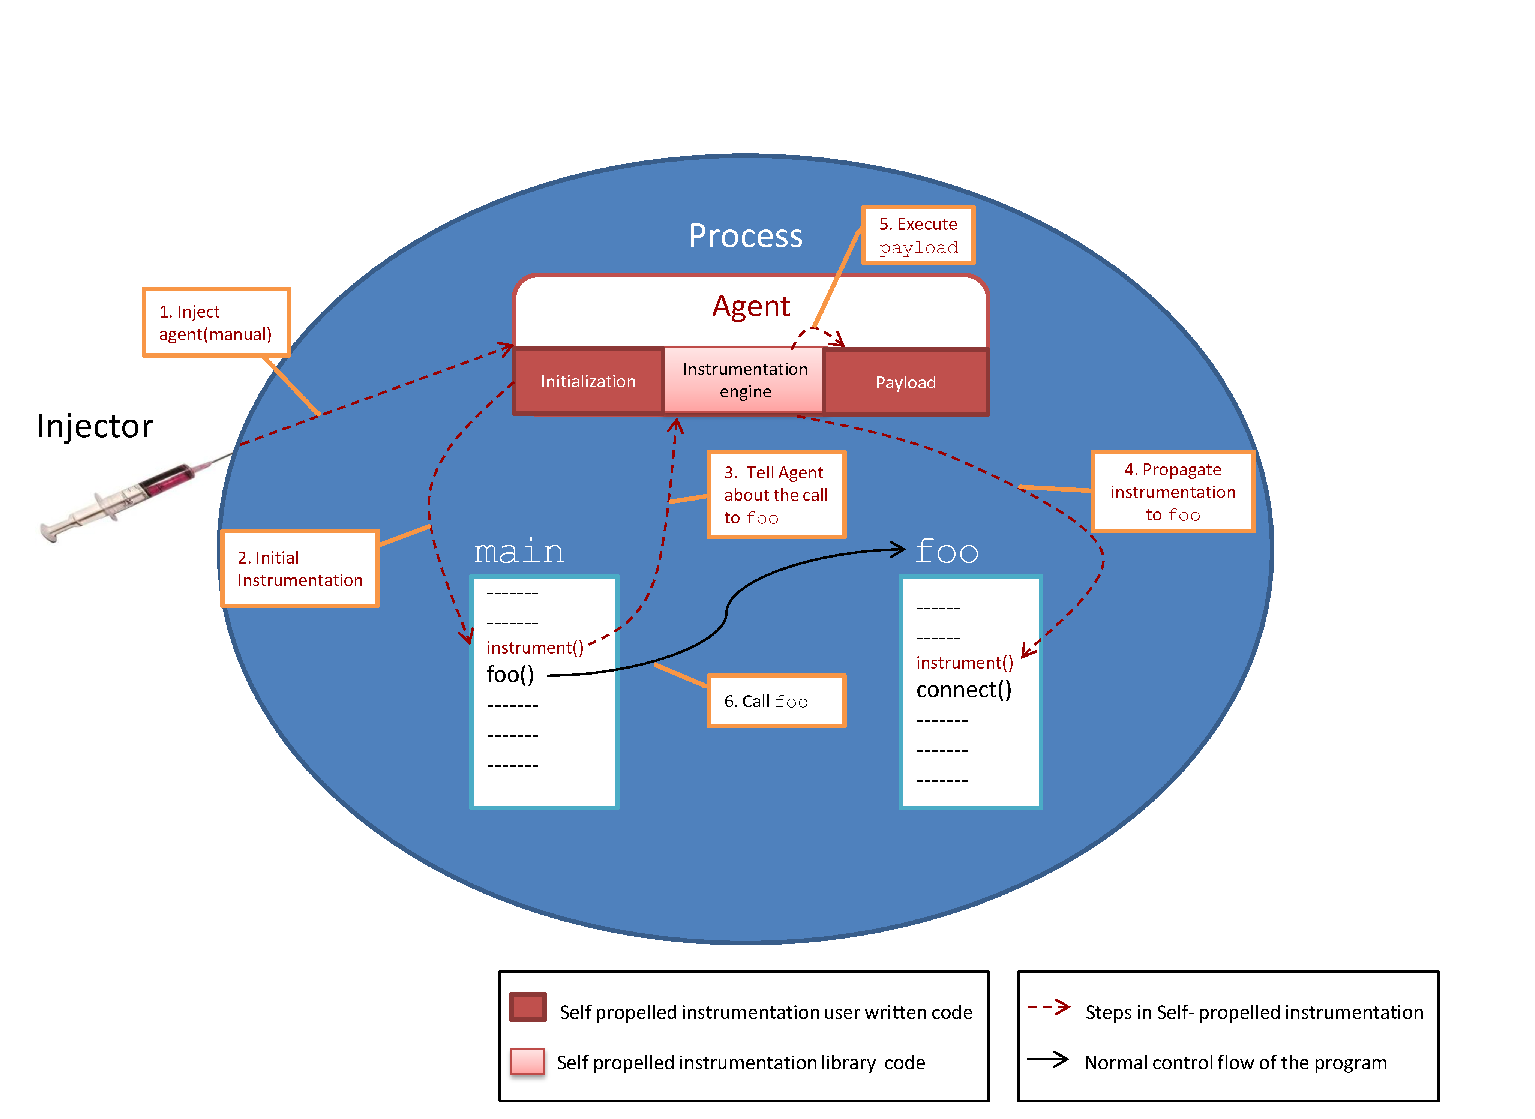
\includegraphics[width=0.90\textwidth]{figure/intraprocess.eps}
  \caption{Intra-process Self-propelled Instrumentation Workflow}
   \label{fig:intrainst}
\end{figure}

Instrumenting all the function calls inside {\em main} function internally calls
the instrumentation engine, before each function call is made.
Instrumentation engine, in turn, propagates the instrumentation to the called
functions by instrumenting all the function calls inside the called function.

The instrumentation engine also executes payload function either before or after
running the instrumented function call depending on whether it is an entry
payload or exit payload function.

The workflow is visualized in Figure~\ref{fig:intrainst}.

\subsubsection{Inter-process propagation}
\begin{figure}[ht]
  \centering
  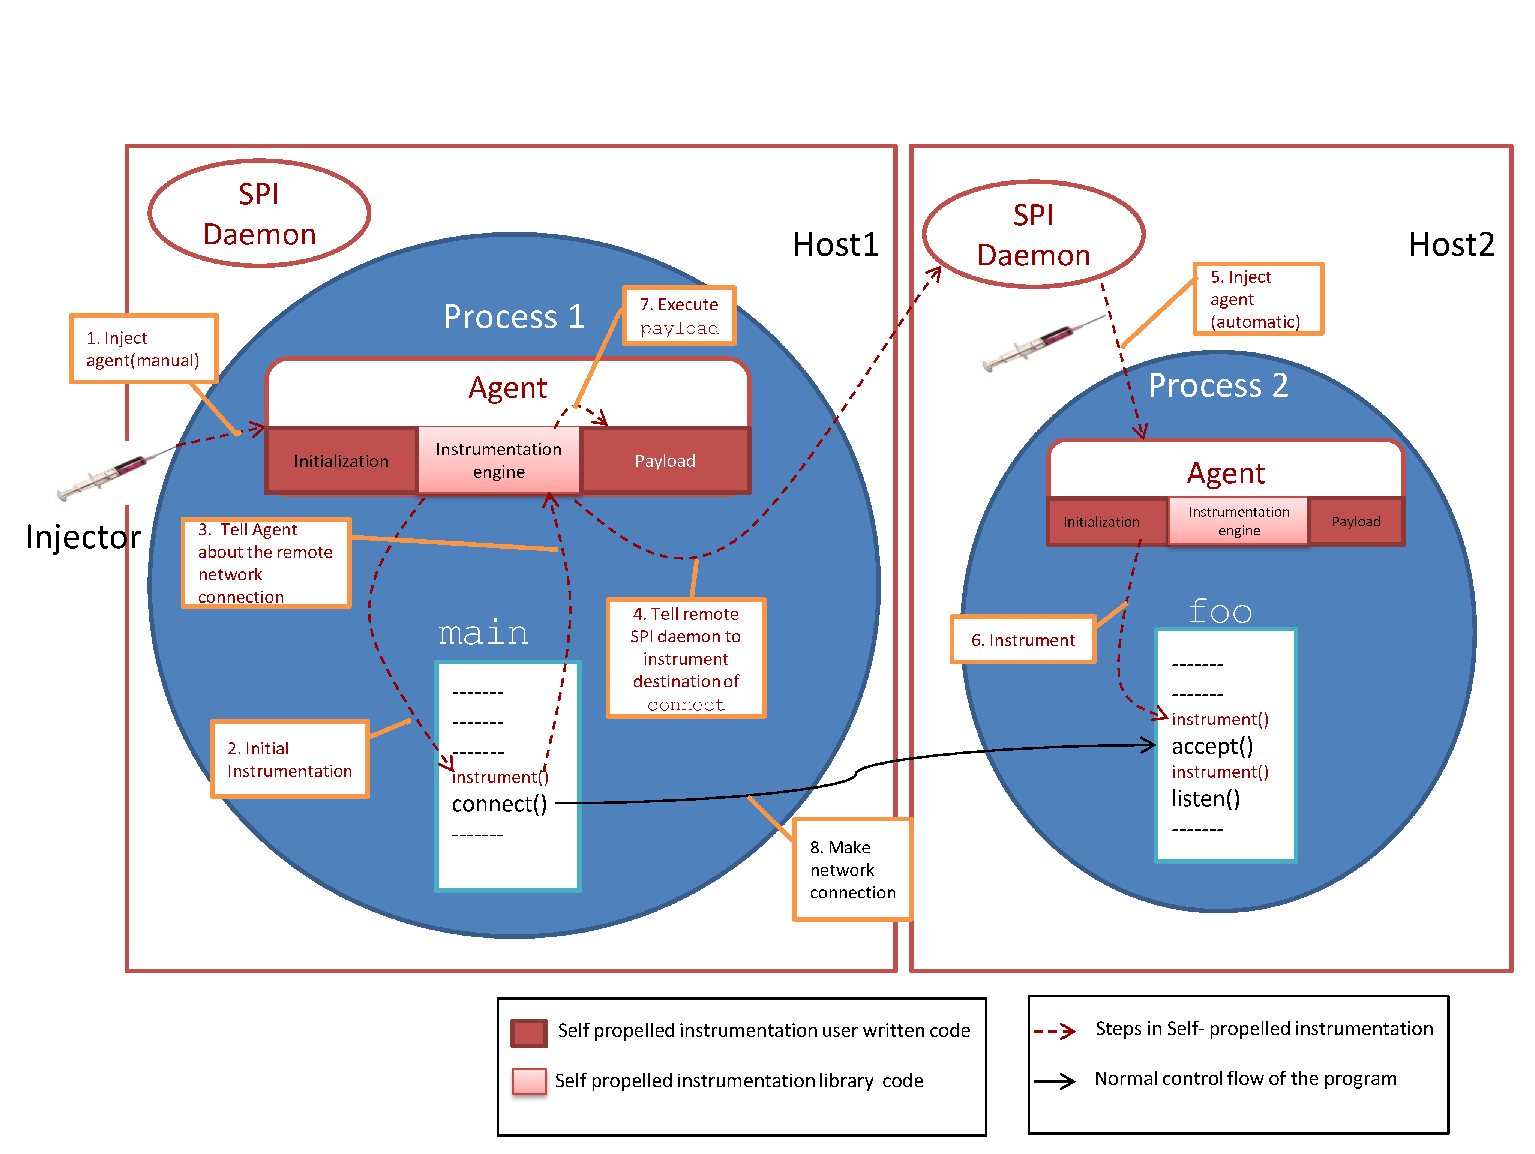
\includegraphics[width=0.90\textwidth]{figure/interprocess.eps}
  \caption{Inter-process Self-propelled Instrumentation Workflow}
  \label{fig:interinst}
\end{figure}

For inter-process instrumentation propagation, the instrumentation engine
identifies communication initiation functions like {\em connect}, {\em send}, or
{\em write} and figures out the target host.
The instrumentation engine then contacts to the SPI daemon of the target host on
the other end of communication, which injects the agent shared library automatically
into the target process. 
Then the usual process of \textit{initialisation} and \textit{initial
  instrumentation} goes on inside the target process. 
The workflow is visualized in Figure~\ref{fig:interinst}
